\question 某个系统采用下列分配策略:如果一个进程提出资源请求得不到满足,若此时没有由于等待该资源而被阻塞的进程,则自己被阻塞;若此时已有因等待该资源而阻塞的进程,则检查所有阻塞进程,如果阻塞进程中持有申请进程所需要的这种资源,则将这些资源剥夺并分配给申请进程。这种分配策略会导致
\par\twoch{死锁}{颠簸}{回退}{\textcolor{red}{饥饿}}
\begin{solution}本题所给的资源分配策略不会产生死锁。因为题中的分配策略规定若一个进程的资源得不到满足,则检查所有由于等待资源而被阻塞的进程,如果它们有申请进程所需要的资源,则将这些资源取出分配给申请进程,从而破坏了产生死锁必要条件中的非剥夺条件,这样系统就不会产生死锁。
但是,这种方法会导致某些进程无限期的等待,即阻塞。因为被阻塞进程的资源可以被剥夺,所以被阻塞进程所拥有的资源数量在其被唤醒之前只可能减少。若系统中不断出现其他进程申请该资源,则这些进程都可能会剥夺阻塞进程的资源,导致阻塞进程会一直由于缺少资源而无限期阻塞,导致饥饿。
因此本题选择D选项。
\end{solution}
\question 某时刻进程的资源使用情况如下表所示。此时的安全序列是(
~)。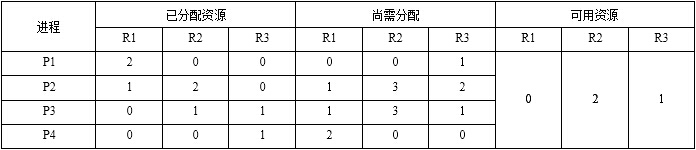
\includegraphics[width=3.33333in,height=0.71875in]{computerassets/42b88243077ecc1d531d920fb4b79fe3.jpeg}
\par\fourch{P1,P2,P3,P4}{P1,P3,P2,P4}{P1,P4,P3,P2}{\textcolor{red}{不存在}}
\begin{solution}使用银行家算法可知,不存在安全序列。由于初始R1资源没有剩余,只能分配资源给P1执行,P1完成之后释放资源。这时由于R2只有2个剩余,因此只能分配对应资源给P4执行,P4完成之后释放资源。此时R2仍然只有2个剩余,无法满足P2、P3的要求,无法分配,因此产生死锁状态。
~ ~ ~
~如果对于银行家算法比较熟悉,能够很快发现R2资源只有2个,但P2和P3的需求都为3,并且P1和P4都没有持有R2资源,R2资源会始终无法满足P2和P3的需求,必然会在若干步分配后导致死锁。
【总结】 ~ ~ ~
~本题相对来说比较简单,每次的分配选择都只有一个,推导两步就可以得到死锁的结果,保证了题目结果的唯一性。在有些比较麻烦的题目中,分配选择会有多个,可能要进行多次尝试才能得到结果。
\end{solution}
\question 假设5个进程P0、P1、P2、P3、P4共享三类资源R1、R2、R3,这些资源总数分别为18、6、22。T0时刻的资源分配情况如上表所示,此时存在的一个安全序列是(
~)\\

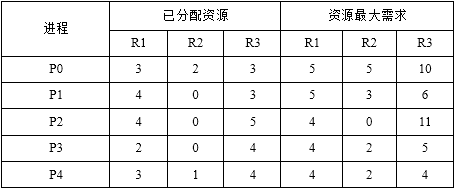
\includegraphics[width=3.12500in,height=1.29167in]{computerassets/87C28FE0EB82CF475B0E849EEE5BB8AC.png}
\par\fourch{P0,P2,P4,P1,P3}{P1,P0,P3,P4,P2}{P2,P1,P0,P3,P4}{\textcolor{red}{P3,P4,P2,P1,P0}}
\begin{solution}对4个选项分别进行安全性检测,只有D选项能够全部执行结束,其他3个选项都不能执行完全,中途会出现资源不足而死锁。
\end{solution}
